\documentclass[pdftex,12pt,a4paper]{article}
\usepackage{amsthm}
\usepackage{amssymb}
\usepackage{enumerate}
\usepackage{amsmath}
\usepackage{verbatim}
\usepackage{graphicx}
\usepackage{hyperref}
\usepackage{fancyhdr}

\newcommand{\HRule}{\rule{\linewidth}{0.5mm}}


\pagestyle{fancy}

\fancyhead[RO,RE]{Peter Zhang and Carl Jackson}
\fancyhead[LO, RE]{Pheme: Birds of a Feather Tweet Together}

\begin{document}
\begin{titlepage}
\begin{center}

% Upper part of the page. The '~' is needed because \\
% only works if a paragraph has started.

\includegraphics[width=0.15\textwidth]{twitterlogo.jpg}~\\[1cm]


\textsc{\Large CS 171: Project 2}\\[0.5cm]

% Title
\HRule \\[0.4cm]
{ \LARGE \bfseries Pheme: \\ Birds of a Feather Tweet Together} \\[0.4cm]

\HRule \\[1.5cm]

% Author and supervisor
\begin{minipage}{0.6\textwidth}
\begin{flushleft} \large
\emph{Authors:}\\
Carl Jackson and Peter Zhang
\end{flushleft}
\end{minipage}
\begin{minipage}{0.4\textwidth}
\begin{flushright} \large
\end{flushright}
\end{minipage}

\vfill

% Bottom of the page
{\large \today}

\end{center}
\end{titlepage}
\tableofcontents
\pagebreak

\section{Introduction}
\subsection{Motivation}
Most current visualizations of social data require viewers to already have a subject matter in mind; they allow viewers to search for and investigate specific keywords, hashtags, or locales. However, we think that social data is interesting primarily because it allows us to discover new topics for investigation - topics that are being generated in real time by the humans who are producing the social data. Accordingly, we want to build a visualization that guides a curious but unfocused viewer in identifying undiscovered topics/events that are currently occurring in the real world.
\subsection{Goals}
In this project, our goal is to investigate high-throughput social data streams, and answer two primary research questions:
\begin{enumerate}
\item Can we identify "events" from real-time social data?
\item If we can, what can we learn about such "events" from various social data sources?
\end{enumerate}
To achieve these goals, we have built a visualization that tries to identify current events that are occurring within a user-specified geography (location + radius), using real time social data. Concretely, we pull a live stream of Twitter data being generated in the specified geography, and try to identify clusters of tweets; currently, we cluster primarily by geographical proximity, but hope to cluster using other techniques in project 3.

\section{Description of Data}
\subsection{Source}
The ultimate source of the data for our visualizations is Twitter, an online social network and microblogging service that allows users to instantaneously send and receive short messages, called tweets, on various electronic devices. Twitter is one of the most popular, if not the most popular, sites that produces real-time social data; as of 2012, it produced more than 340 million tweets per day \footnote{http://techcrunch.com/2012/07/30/analyst-twitter-passed-500m-users-in-june-2012-140m-of-them-in-us-jakarta-biggest-tweeting-city/}. Given our interest high-throughput social data streams, Twitter was a natural data source to focus on.

Using Twitter's API, we pulled tweets, which contained several relevant pieces of information:
\begin{enumerate}
\item Geographical location: Twitter users can choose to specify a geographical location to associate with their tweet. This is particularly interesting for users who tweet on their mobile phones, and choose to expose their phone's GPS data to the service.
\item Twitter Screenname: Tweets are associated with the screen name of the user publishing the tweets.
\item Tweet contents: The actual text content of the tweet. This is also available to viewers of our visualization.
\item Hashtags: Twitter users can specify hashtags, or metadata, to associate with their tweet. 
\item Tweet timestamp: The time at which the tweet was published.
\end{enumerate}

\subsection{Scraping Method}
For Carlllllll. Tell story like this:
\begin{enumerate}
\item Normal twitter stream is all historical.
\item Want realtime twitter data.
\item Lots of realtime twitter data doesn't have geographical data, which is essential; how did you solve?
\item Challenge where you could only pull from certain locations.
\item Fix of that bug.
\item Any other challenges you can think of.
\end{enumerate}

\section{Related Work}
To the extent that we've used what we've learned so far in CS 171, all the readings and lecture materials are related work; when justifying our visualization choices or visualization evolution, we will refer to this material. We consulted documentation related to the Twitter API and the Google Maps API very often while working on this project. Finally, we were inspired to investigate and study tweets and their geographical data by a past CS 171 project: Tweetography. \\ \\
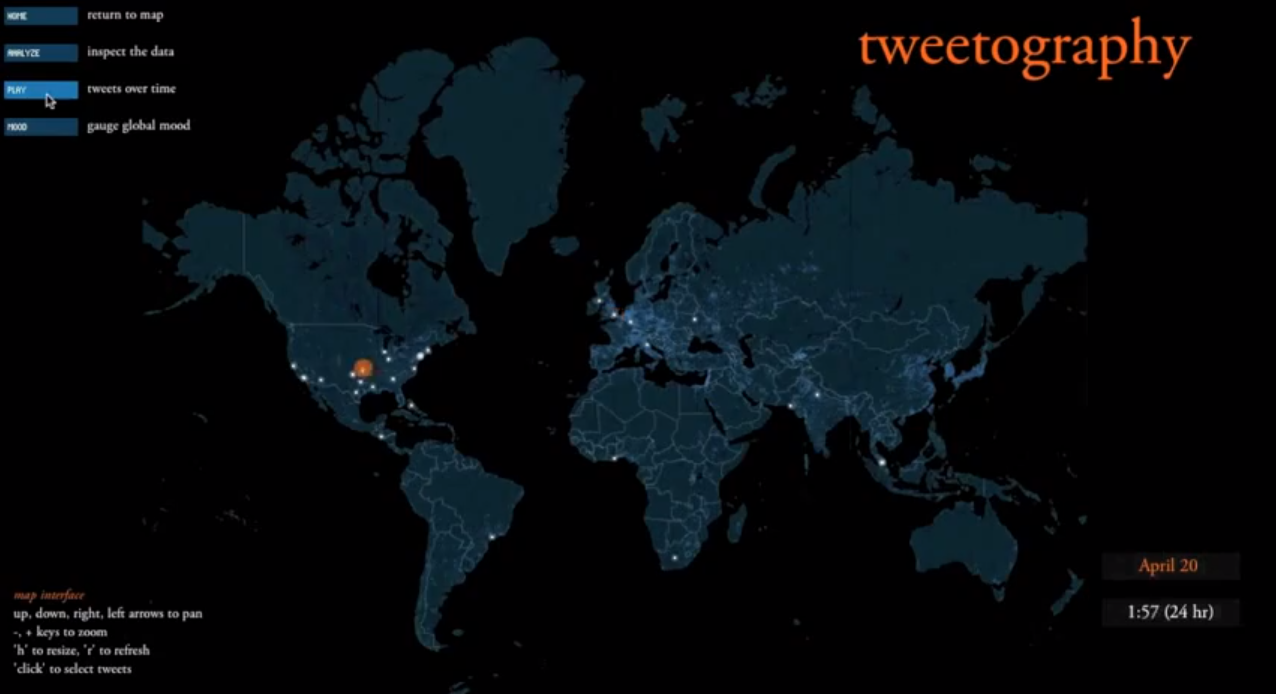
\includegraphics[width=5.5in]{tweetography.png} \\ \\
We found the concept of tweets appearing over time on a map very attractive, and based our visualization on this concept, even though the purpose and design of our visualization is very different than Tweetography.

\section{Design Evolution}
In our initial proposal, we envisioned a visualization where tweets, and clusters of tweets that have been identified as a cluster, are displayed on a map as they are generated; our initial sketch of how this might look is included below: \\ \\
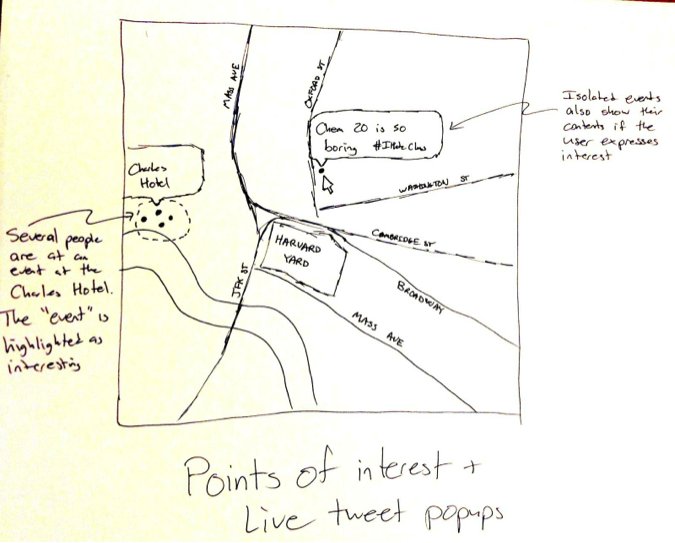
\includegraphics[width=5in]{proposal1.png} \\ \\
In addition, we imagined a sidebar that would display tweet and cluster information as they came in, similar to the image below: \\ \\
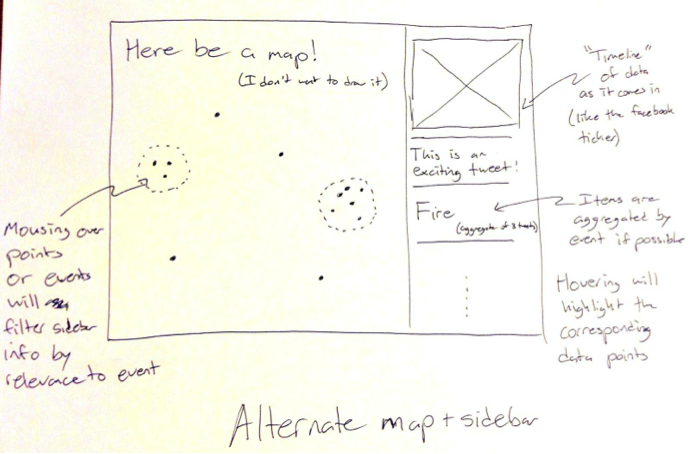
\includegraphics[width=5in]{proposal2.png} \\ \\
Throught the evolution of our visualization, these fundamental design choices have not changed. However, we did have to address specific design issues during this project.

\subsection{Maps}
First, we had to decide on the background of our visualization, the map. As covered in class and homework, there are several ways to draw maps using D3, including an SVG map from wikipedia or the datamaps add-on. We really liked D3, especially the way it binds data directly to elements of the DOM. However, we ultimately decided that D3 was not particularly suitable for our visualization, because we needed a very finely detailed map for our visualization. Since we desired to identify events and their geographical location, it was important for users to be able to see the exact street address of the tweets and events we were visualizating, as well as the surrounding buildings and other geographical features. For example, one event we ultimately identified while testing our visualization was the opening game at Fenway Park: \\ \\
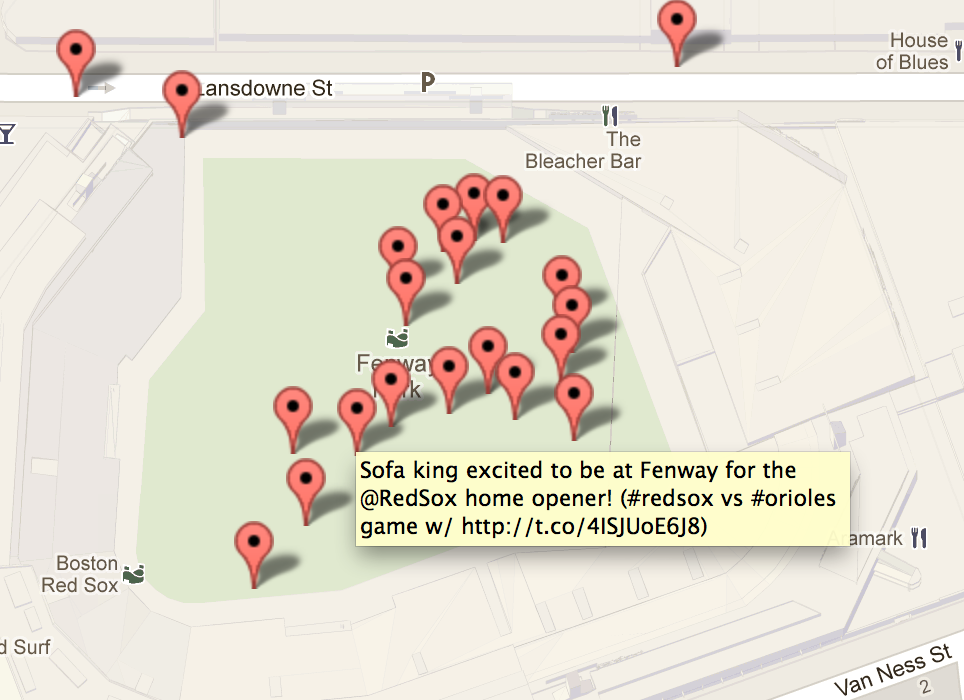
\includegraphics[width=5.5in]{fenway.png} \\
If the map we chose to visualize tweets on did not contain detailed city, street, and building information, it would have been much harder to understand exactly what and where this event was occurring.
Accordingly, we decided to build our visualization using the Google Maps API. In addition to a very detailed map, which would help viewers make a variety of useful visual queries relating to the events we identify, the Google Maps API contains several nice features, including zooming - which will allow users to drill down/filter as we explain later - and simple methods to draw basic objects on the map. 

\subsection{Clustering}
We faced several challenges when deciding how to construct and visualize our clusters.



\section{Visualizations} 


\subsection{Clustering}

\subsection{Colors} 
\section{Conclusion}
Through this process of Exploratory Data Analysis, I've identified several interesting relationships between game usage statistics and various game attributes, as well as relationships between different game attributes. That being said, if I had more time, I would be interested in further investigating this data in the following ways:
\begin{enumerate}
\item Examine the relationship between hourly game usage statistics and price, language count, ESRB rating, metacritic rating, etc.
\item Identify any differences between hourly game usage statistics on week and weekend days.
\item Scrape data for games other than games in the top 100 games by current user count, to get a richer picture of how various game attributes affect to each other.
\end{enumerate}
Furthermore, number 3 on this list emphasizes a general weakness with the data I used: I only collected data for the top 100 games by current user count at the current date and time. This data collection method likely introduced some artifacts into the data, like the dropoff of current users playing racing games to zero at certain times of day, and thus all results presented above should be regarded with caution; further investigation is needed to confirm these trends. 
\end{document}